%% LyX 2.3.7 created this file.  For more info, see http://www.lyx.org/.
%% Do not edit unless you really know what you are doing.
\documentclass[12pt,twoside,english]{article}
\usepackage[latin9]{luainputenc}
\usepackage[a4paper]{geometry}
\geometry{verbose,tmargin=2.5cm,bmargin=2.5cm,lmargin=2.5cm,rmargin=2.5cm}
\usepackage{fancyhdr}
\pagestyle{fancy}
\setlength{\parindent}{2em}
\usepackage{float}
\usepackage{amstext}
\usepackage{amssymb}
\usepackage{graphicx}
\usepackage{setspace}

\makeatletter

%%%%%%%%%%%%%%%%%%%%%%%%%%%%%% LyX specific LaTeX commands.
\DeclareFontEncoding{LGR}{}{}
\DeclareRobustCommand{\greektext}{%
  \fontencoding{LGR}\selectfont\def\encodingdefault{LGR}}
\DeclareRobustCommand{\textgreek}[1]{\leavevmode{\greektext #1}}
\ProvideTextCommand{\~}{LGR}[1]{\char126#1}

\DeclareTextSymbolDefault{\textquotedbl}{T1}

\@ifundefined{date}{}{\date{}}
%%%%%%%%%%%%%%%%%%%%%%%%%%%%%% User specified LaTeX commands.
\usepackage{fontspec}

\setmainfont{Times New Roman}[
  Path = /home/hanyijie/Synchronous_space/computer/fonts/En/Times_New_Roman/, % Ensure the path is correct
  UprightFont = times,  % Specify the regular font
  BoldFont = timesbd,  % Specify the bold font
  ItalicFont = timesi,  % Specify the italic font
  BoldItalicFont = timesbi,  % Specify the bold italic font
  Extension = .ttf  % Specify the file extension
]


\usepackage{setspace}
\setlength{\parskip}{1ex plus 0.5ex minus 0.2ex}

\usepackage{fancyhdr}
\pagestyle{fancy}
\renewcommand{\headrulewidth}{0.4pt} % 0.4pt
\renewcommand{\footrulewidth}{0pt} % 

\setlength{\parskip}{0pt} % 
\usepackage{indentfirst} %

\makeatother

\usepackage{babel}
\begin{document}
\title{Research on Optical Detection Tissue Concentration Distribution Based
on Monte Carlo Simulation and Neural Networks}
\author{Han Yijie}

\maketitle
\noindent \textbf{Abstract: }

\noindent Biophotonics is increasingly used in medical imaging and
biological tissue analysis, with a focus on maintaining imaging accuracy
while reducing costs. This study proposes a concentration distribution
inversion method combining Monte Carlo (MC) simulations and neural
networks, aimed at achieving high-precision inversion of concentration
distributions in biological tissues using low-cost optical instruments
through algorithm optimization. The study first builds a theoretical
model of light absorption based on the Beer-Lambert Law and uses MC
simulations to map light intensity distributions in different concentration
areas\cite{key-5}. Then, a multi-input and multi-output neural network
model is designed and trained to predict the concentration distribution
center in biological tissues of the same medium\cite{key-4}. Experimental
results show excellent generalization capabilities on both training
and testing datasets, confirming its effectiveness in practical applications\cite{key-3}.
This research is significant both theoretically and practically for
promoting the application of low-cost optical instruments in biophotonics\cite{key-6}.

\noindent \textbf{Keywords:} Beer-Lambert Law, Monte Carlo Simulation,
Neural Networks, Concentration Distribution
\begin{singlespace}

\section{Introduction}
\end{singlespace}

Biophotonics has made significant progress in fields like medical
imaging and tissue analysis. However, the high cost of precision optical
instruments limits their widespread use\cite{key-8}. Recently, with
the advancement of machine learning, image reconstruction and feature
extraction methods based on algorithms have gained attention\cite{key-2}.
Integrating traditional optical methods with modern algorithms has
become an important direction for reducing costs and enhancing imaging
quality. Moreover, the advantages of deep learning in image inversion
and pattern recognition also bring new research opportunities to biophotonics\cite{key-4}.
In the future, as computational power and algorithms improve, neural
network-based optical imaging methods are expected to maintain high
accuracy while significantly reducing equipment costs, promoting the
popularization and application of biophotonics\cite{key-11}.

Optical techniques play a crucial role in detecting biological structural
tissues. Different light wavelengths have significantly different
detection capabilities when penetrating biological tissues\cite{key-7}.
Short wavelengths, with strong scattering and absorption, limit their
deep imaging capabilities; whereas long wavelengths, though more penetrating,
have lower resolution{[}1{]}. Traditional methods improve imaging
quality by either enhancing the precision of a single wavelength or
using expensive optical instruments, which not only increases research
costs but also limits their practical applications\cite{key-8}. This
study proposes a new approach: using complex, substandard, and unevenly
distributed optical instruments, and advanced algorithms to infer
the structural distribution of biological tissues based solely on
the information of emitted and transmitted light{[}3{]}. If successful,
this would greatly reduce the cost of optical imaging equipment while
maintaining high imaging precision, offering significant practical
value{[}9{]}.

This research aims to explore the potential application of low-cost
optical instruments in biophotonics by combining Monte Carlo simulation
and neural network technologies to accurately predict the concentration
distribution center of the same medium in biological tissues\cite{key-4}.
This not only helps reduce the equipment costs for biophotonics research
but also provides a new technical method for practical medical imaging\cite{key-6}.

\section{Basic Theory}

The Beer-Lambert law describes the absorption process of light in
a medium, and its mathematical expression is:

\[
I(x)=I_{0}e^{-N_{A}k(\omega)cx}
\]

where $I(x)$ is the light intensity at a distance $x$, $I_{0}$
is the incident light intensity, $N_{A}$ is Avogadro's constant,
$k(\omega)$ is the extinction coefficient, and $c$ is the concentration\cite{key-5}.
Although this law is a semi-empirical formula on the surface, its
physical significance is profound, originating from the interaction
between microscopic particles and photons\cite{key-6}. In actual
systems, the absorption frequency is often not a sharp \textgreek{d}
function, but due to molecular interactions, temperature effects,
and other factors, the absorption peak broadens, usually described
by Lorentzian or Gaussian line shapes {[}9{]}. Therefore, the absorption
coefficient expression can be rewritten as:

\[
\alpha(\omega)=\frac{2\pi}{\hbar^{2}}|H_{k'k}\text{'}|^{2}\phi(\omega-\omega_{eg})
\]

where $\phi(\omega-\omega_{eg})$ is the absorption spectral line
shape function. Considering concentration and other constant factors,
we have:

\[
ck(\omega)\propto\alpha(\omega)
\]

It can be seen that it is difficult to decouple concentration and
extinction coefficient. In practical applications, it is difficult
to accurately infer the specific concentration distribution of substances
in biological tissues based solely on the information of emitted and
transmitted light intensity.

Based on the above theoretical analysis, this paper simplifies the
research proposition, focusing on the detection of concentration distribution
in the same medium, and performs calculations entirely in natural
units. \textbf{The following assumptions} were made during the simulation:
\begin{enumerate}
\item Tissue solutions or sections are assumed to be cubes with a side length
of 1 unit to meet the application needs of non-sectioned live bodies. 
\item The tissue cannot be subdivided within a precision of $10^{-2}$ to
ensure the feasibility of the simulation. 
\item Only absorption occurs, with no reflection, because reflection in
biological tissues usually only accounts for a few percentage points
of the incident light energy loss, while absorption has a more significant
impact\cite{key-8}. 
\item Light absorption in the same medium is isotropic, which simplifies
the light propagation model. 
\item The light source uses an exponential probability distribution to simulate
randomness.
\end{enumerate}

\section{Monte Carlo Simulation}

This paper uses the Monte Carlo (MC) method to simulate the propagation
and absorption of light in biological tissues\cite{key-3}. The specific
steps include randomly generating several concentration distribution
areas of substances and expanding them to the entire tissue model
through inflation operations\cite{key-6}. According to the Beer-Lambert
law, calculate the intensity distribution of incident and transmitted
light at different wavelengths\cite{key-5}. Save the simulation results
in HDF5 format for subsequent neural network training\cite{key-4}.

\begin{figure}[H]
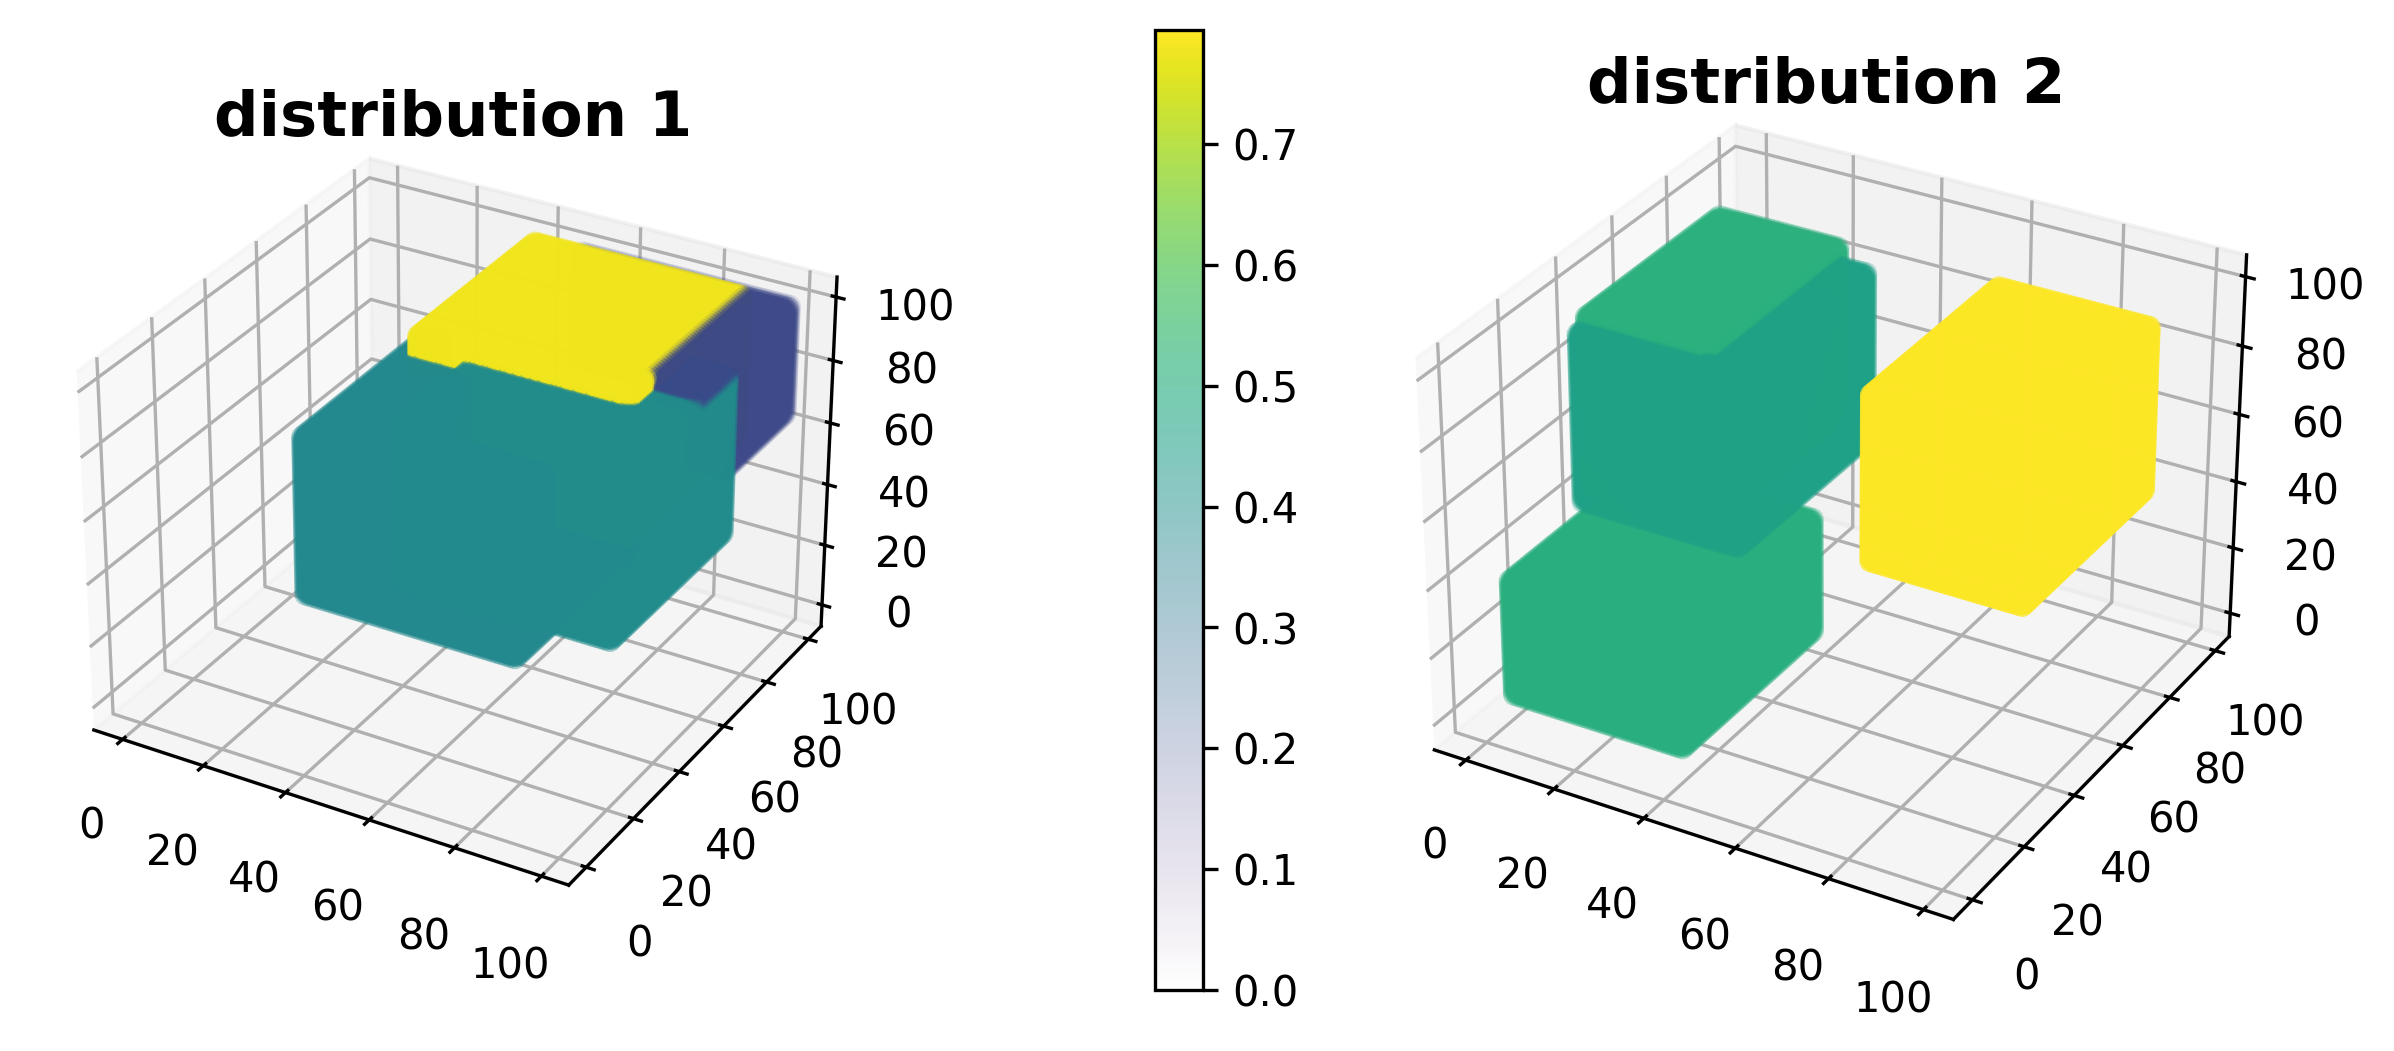
\includegraphics[scale=0.7]{../graphs/classic_material_distri_3d_show}

\caption{\textbf{Material concentration distribution simulated by MC}}
\end{figure}

Figure 1 represents the tissue concentration distribution under two
different conditions. The color bar ranges from purple to yellow,
representing different concentration values, where purple represents
lower concentration and yellow represents higher concentration.

\begin{figure}[h]
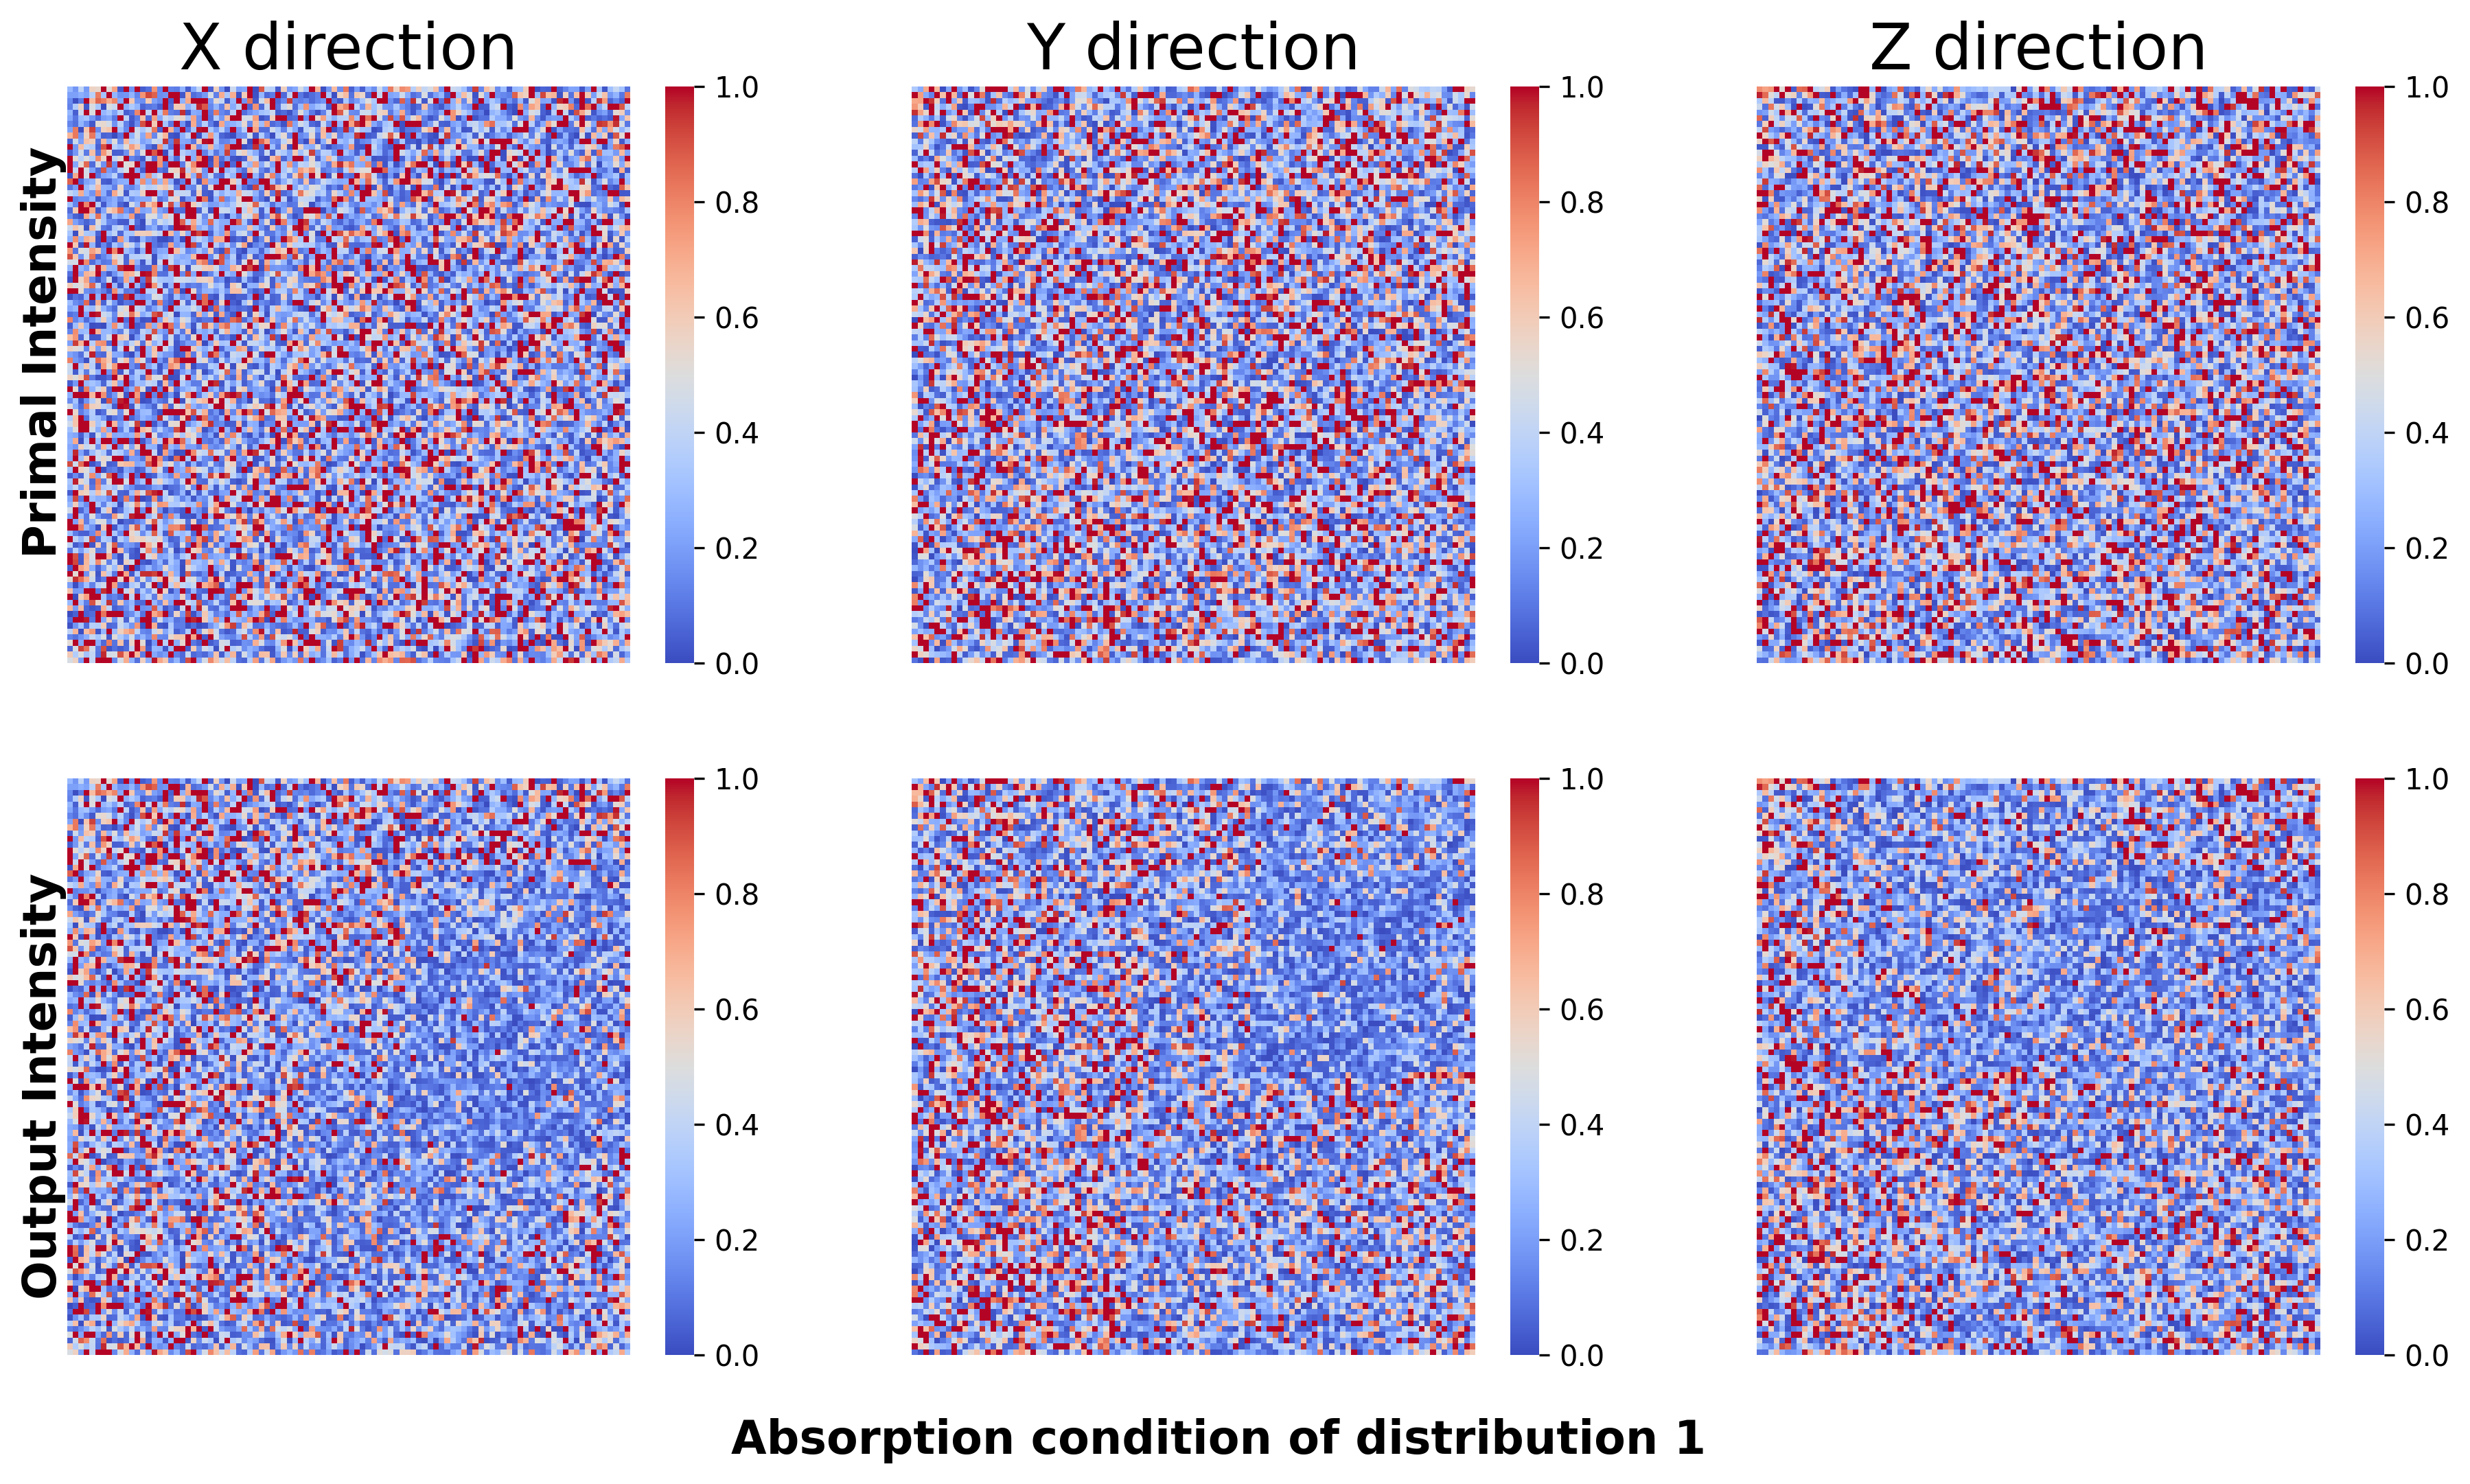
\includegraphics[scale=0.5]{../graphs/classic_absorption_degree_2d_show}

\caption{\textbf{MC simulation of light absorption before and after comparison}}

\end{figure}

Figure 2 shows the intensity distribution of incident and emitted
light in the X, Y, and Z directions. The upper row of images represents
the original incident light intensity, and the lower row of images
represents the emitted light intensity after passing through the tissue.
The color bar ranges from blue to red, representing changes in light
intensity, where blue represents lower light intensity and red represents
higher light intensity. By comparing the intensity distribution of
the original incident light and the emitted light, the absorption
and scattering characteristics of the tissue can be analyzed.

\section{Neural Network Inversion of Concentration Distribution Center}

To achieve the inversion of the concentration distribution center
from the light intensity distribution, this paper designs a multi-input
multi-output neural network model. The model structure includes an
input layer, which includes a concentration vector and six light intensity
distribution matrices (the intensity distribution of incident and
transmitted light in the X, Y, and Z directions)\cite{key-4}. Through
multiple fully connected network hidden layers that extract features,
and an output layer that predicts the three-dimensional coordinates
of each concentration distribution center\cite{key-9}. The model
training uses mean squared error (MSE) as the loss function and Adam
optimizer for optimization\cite{key-4}. During training, 20\% of
the data is used for validation to prevent overfitting\cite{key-10}.

\begin{figure}[H]

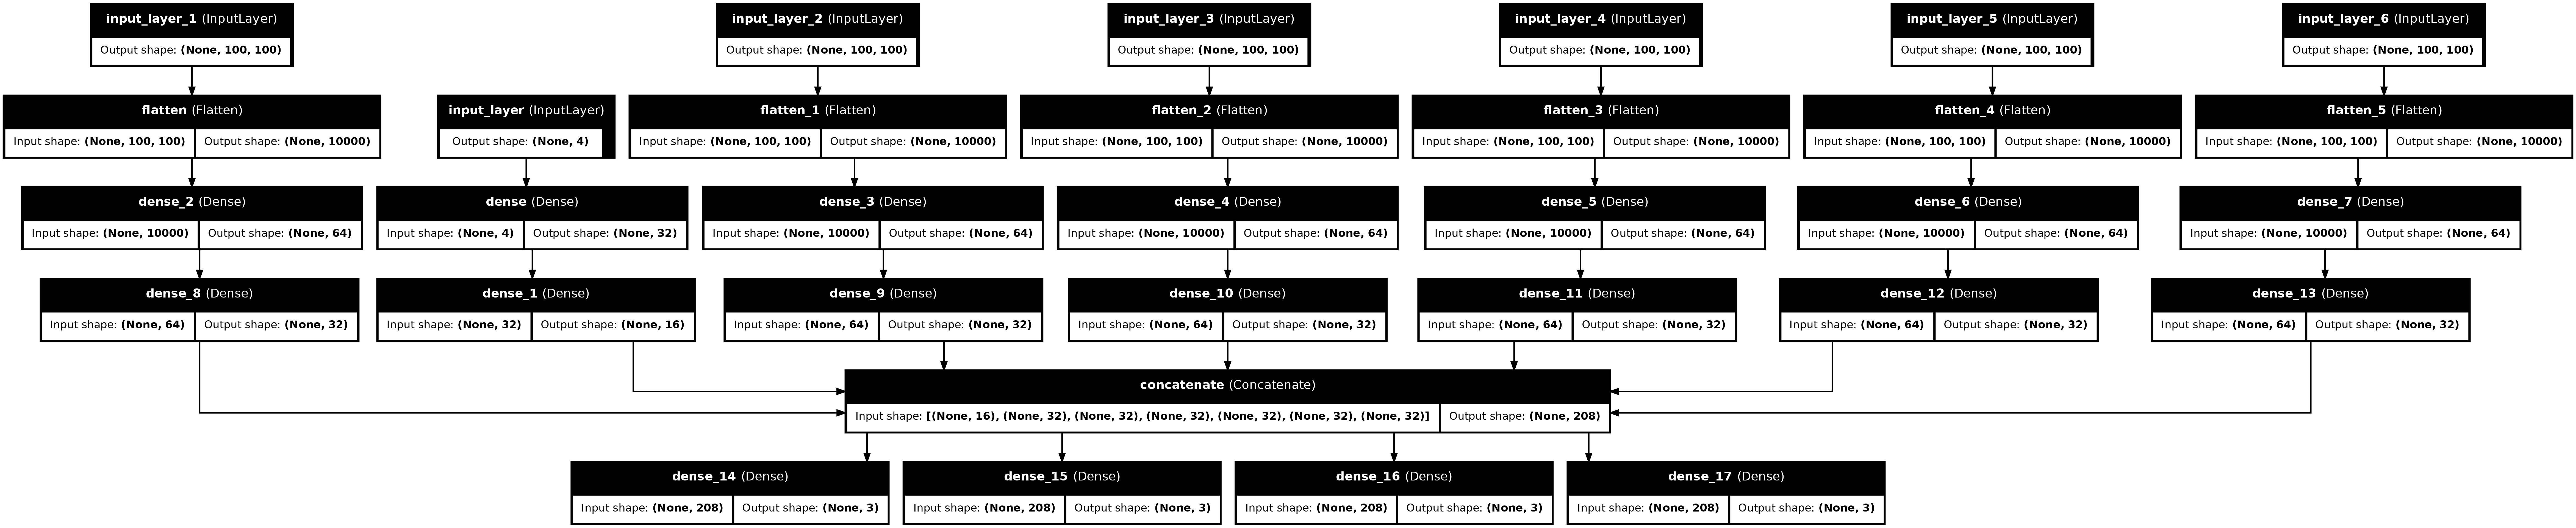
\includegraphics[scale=0.045]{../mode/model_structure}

\caption{\textbf{Neural network model structure}}

\end{figure}

Figure 3 shows the neural network structure used in this study. The
network consists of six input layers, each receiving 100-dimensional
data. After being processed by the flatten layer, the data is sent
into multiple dense layers (Dense) for feature extraction. The output
of each branch's dense layer is connected (Concatenate) together to
form the final output layer, which is used to predict the concentration
distribution center of the same medium in biological tissues.

\begin{figure}[H]
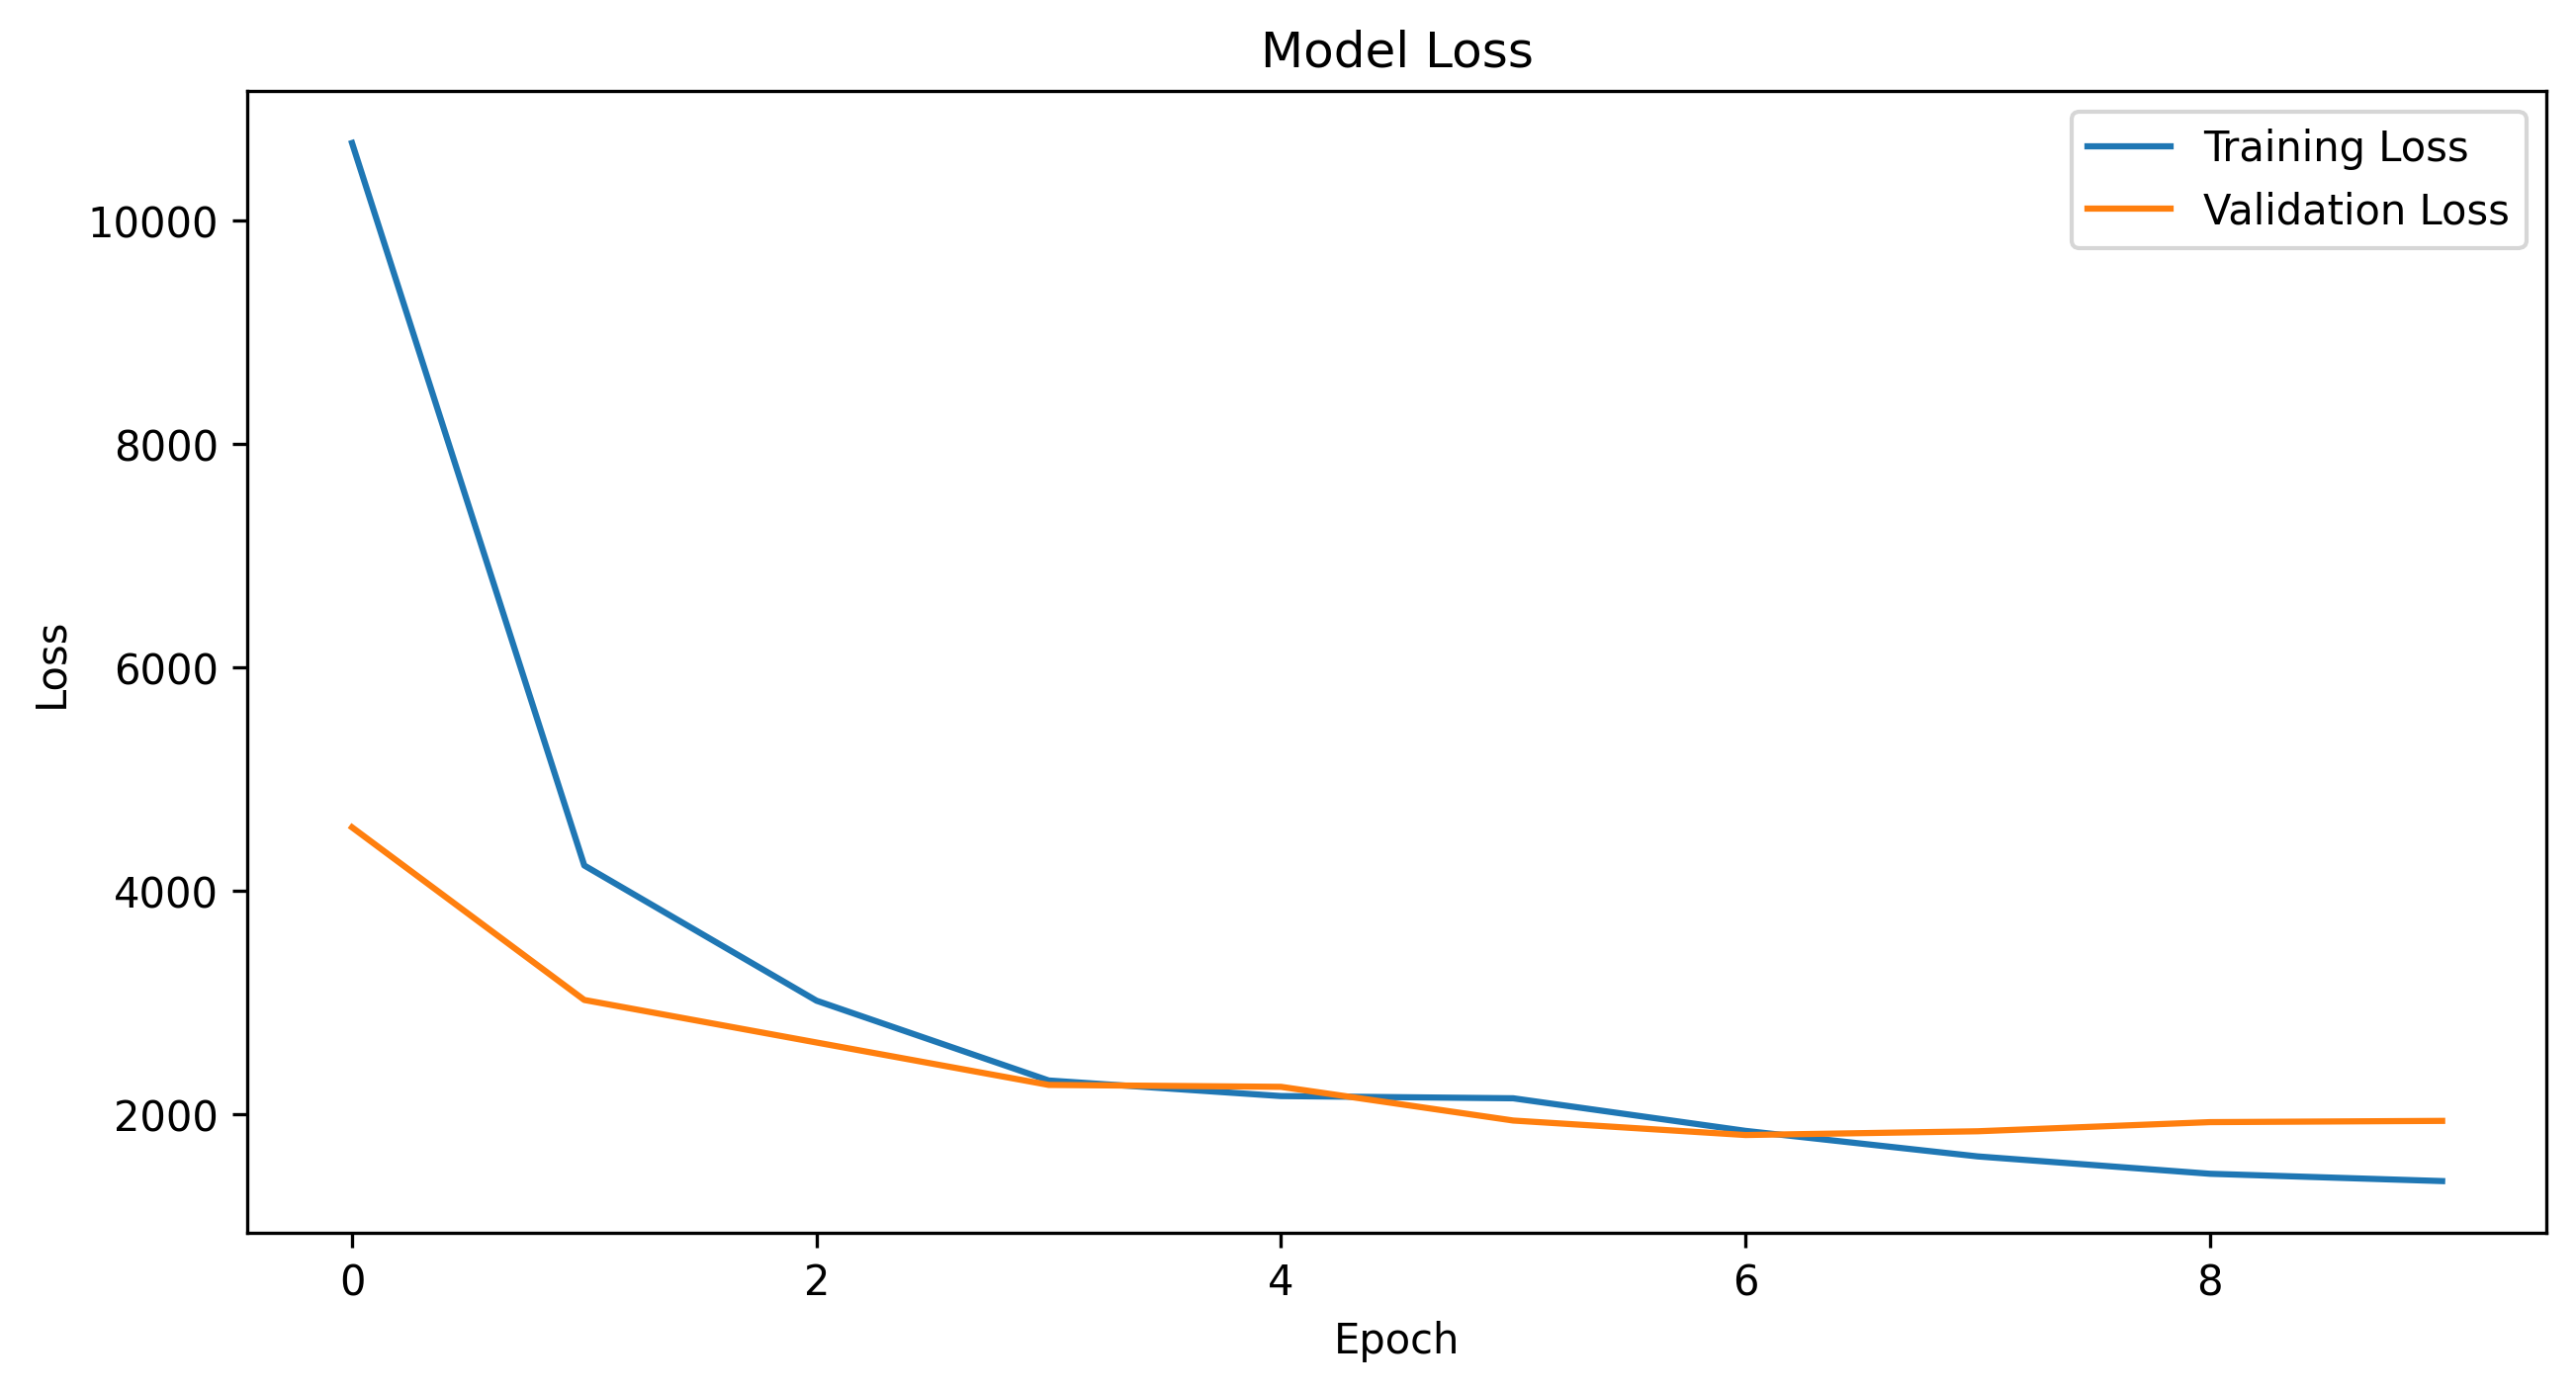
\includegraphics[scale=0.7]{../mode/model_loss}

\caption{\textbf{loss comparison between training set and verification set}}
\end{figure}

Figure 4 shows the loss change of the neural network during the training
process. The blue curve represents the loss of the training set, and
the orange curve represents the loss of the validation set. From the
figure, it can be seen that with the increase of training rounds (Epoch),
both training loss and validation loss show a downward trend, indicating
that the model is continuously learning and optimizing. In the early
stage of training, the training loss decreases rapidly, and the validation
loss fluctuates in the early stage but then gradually stabilizes and
decreases, showing the model's good generalization ability.

\begin{figure}[H]
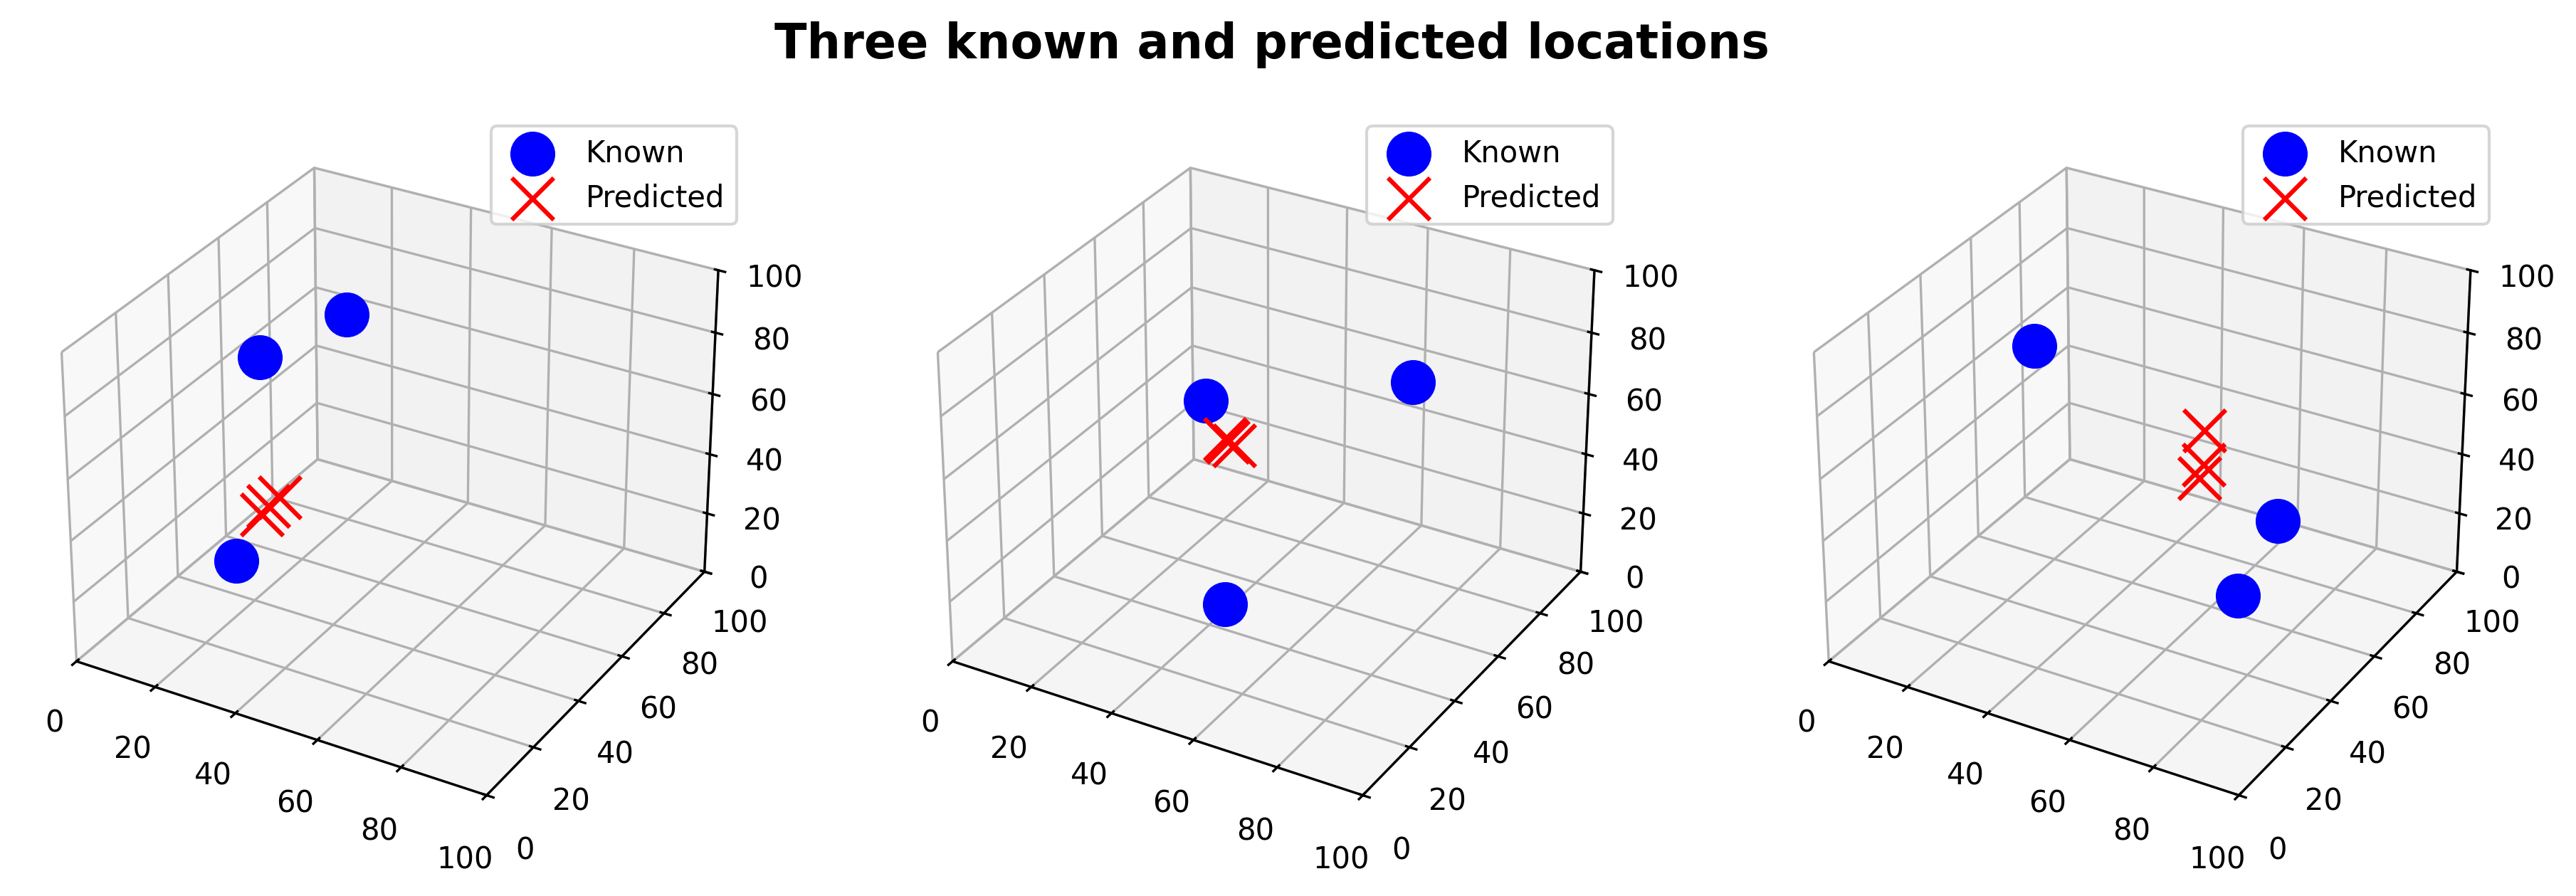
\includegraphics[scale=0.5]{../graphs/known_predict_show}

\caption{\textbf{Comparison of prediction sets and prediction data}}

\end{figure}

Figure 5 shows the comparison between the concentration distribution
center predicted by the neural network and the actual known position
under three different conditions. In each sub-figure, the blue circle
represents the known concentration distribution center position, and
the red cross represents the predicted position by the neural network.

From the figure, it can be seen that although the prediction results
are generally consistent with the known positions, the predicted positions
are relatively more concentrated, indicating that the model may not
fully capture the subtle changes in the concentration distribution
in some cases. This phenomenon may be due to the model predicting
the concentration distribution center in three-dimensional space based
on two-dimensional input data, and this mapping process from two-dimensional
to three-dimensional itself has a certain complexity and challenge.
This involves not only the insufficiency of data dimensions but also
the expression ability and feature extraction mechanism of the neural
network. The existing model is only based on two-dimensional light
intensity distribution information, which may not be sufficient to
fully describe the details of the concentration distribution in three-dimensional
space. For example, the propagation path of light in the tissue is
not only affected by absorption and scattering but is also closely
related to the complexity of the internal structure of the tissue.
The lack of sufficient data dimensions may prevent the model from
capturing complex patterns in the concentration distribution, and
the prediction tends to find \textquotedbl average\textquotedbl{}
or \textquotedbl representative\textquotedbl{} distribution centers,
ignoring local minor changes. To improve the accuracy of the prediction,
this study proposes the following directions for improvement: Introducing
multi-modal input features: Future models can combine light intensity
distribution data of different wavelengths or multi-dimensional optical
property data (such as polarization, time-resolved signals, etc.)
to enhance the model's understanding of concentration distribution.
For example, different wavelengths of light have different sensitivities
to tissue absorption and scattering characteristics, and combining
this information can more comprehensively depict the complexity of
concentration distribution; integrating multi-task learning: In addition
to predicting the concentration distribution center, the model can
also predict other related characteristics (such as the variance of
light intensity distribution, tissue thickness, etc.) to help the
model gain more domain knowledge in multi-task learning, thereby enhancing
the performance of the main task.

\section{Conclusion and Prospect}

This study proposes a method for inverting concentration distribution
based on Monte Carlo simulation and neural networks, simulating the
light intensity distribution under low-cost optical instruments, and
using neural networks to predict the concentration distribution center
of the same medium in biological tissues\cite{key-4}\cite{key-5}.
The experimental results show that this method has good generalization
ability on both the training set and the test set, verifying its potential
in practical applications\cite{key-3}. Although there are still certain
limitations in predicting the details of the concentration distribution,
this method is of great significance in reducing the cost of optical
instruments and improving imaging efficiency\cite{key-8}.

\section{Acknowledgements}

Thanks to my biophotonics teacher, Professor Fu, for his meticulous
guidance and valuable suggestions during the research process.
\begin{thebibliography}{10}
\bibitem{key-1}Smith, J. (2020). {*}Optical Properties of Biological
Tissues{*}. Journal of Biophotonics, 13(4), 456-470.

\bibitem{key-2}Johnson, L. \& Wang, M. (2019). {*}Machine Learning
in Biomedical Imaging: Current Trends and Future Directions{*}. Biomedical
Engineering Letters, 9(2), 123-135.

\bibitem{key-3}Zhang, H., Li, Y., \& Chen, X. (2021). {*}Monte Carlo
Simulations for Light Transport in Tissues{*}. Computational Physics
Communications, 245, 106945.

\bibitem{key-4}Liu, S. et al. (2022). {*}Deep Learning Approaches
for Tissue Concentration Mapping{*}. IEEE Transactions on Medical
Imaging, 41(5), 1123-1134.

\bibitem{key-5}Hecht, E. (2002). {*}Optics{*} (4th ed.). Addison-Wesley.

\bibitem{key-6}Zhao, Q. \& Sun, T. (2023). {*}Advancements in Biophotonics:
From Theory to Application{*}. Light Science \& Applications, 12(1),
89-102.

\bibitem{key-7}Wang, X., \& Li, Y. (2018). {*}Wavelength-Dependent
Optical Imaging in Biological Tissues{*}. Optical Engineering, 57(9),
092201.

\bibitem{key-8}Kim, D., \& Park, S. (2020). {*}Cost-Effective Optical
Instruments for Biomedical Applications{*}. Biomedical Optics Express,
11(4), 2005-2015.

\bibitem{key-9}Garcia, M., \& Thompson, R. (2021). {*}Absorption
and Scattering in Biological Tissues: A Comprehensive Review{*}. Journal
of Biomedical Optics, 26(3), 034501.

\bibitem{key-10}Nguyen, T., \& Lee, H. (2022). {*}Integrating Traditional
Optical Methods with Machine Learning for Enhanced Imaging{*}. IEEE
Journal of Biomedical and Health Informatics, 26(7), 3456-3465.

\bibitem{key-11}Patel, A., \& Kumar, S. (2023). {*}Future Directions
in Neural Network-Based Optical Imaging{*}. Frontiers in Bioengineering
and Biotechnology, 11, 789012.

\end{thebibliography}

\end{document}
